\documentclass{beamer}
\usepackage[portuguese]{babel}
\usepackage{listings}
\usepackage{algpseudocode}
\usepackage{xcolor}
\usepackage{amsmath}
\usepackage{amssymb}

\lstset{basicstyle=\ttfamily\footnotesize,breaklines=true}

\usetheme{Pittsburgh}

\usecolortheme{default}
\title[Short Title]{Séries 5}
\author{João Guilherme Iwo De La Costa\\Rogério Camilo dos Santos\\Victor Jorge Carvalho Chaves}
\institute{Conexão dos Garfos}

\begin{document}

\frame{\titlepage}

\begin{frame}
\frametitle{Sumário}
\tableofcontents
\end{frame}

\section{Generalização dos Cubos}

\begin{frame}{Definições}
    \begin{itemize}
        \item Conjunto de cores: $C = \{c_1, c_2, c_3, c_4\}$.
        \item Conjunto de cubos: $Q = \{q_1, q_2, q_3, q_4\}$.
        \item Cada cubo possui 3 pares de faces opostas.
        \item Cada par gera uma aresta no grafo.
    \end{itemize}
\end{frame}

\begin{frame}{Construção do Grafo}
    \begin{itemize}
        \item Grafo $G = (V, E)$, onde:
        \begin{itemize}
            \item $V = C$ (vértices representam cores);
            \item $E = \bigcup_{i=1}^4 E_i$;
            \item Cada $E_i$ contém 3 arestas do cubo $q_i$.
        \end{itemize}
        \item Aresta: $(u, v, i)$
        \begin{itemize}
            \item $u, v \in V$ (pares de cores nas faces opostas);
            \item $i$ identifica o cubo.
        \end{itemize}
        \item Autociclos permitidos.
    \end{itemize}
\end{frame}


\begin{frame}{Objetivo do Problema}
    \begin{itemize}
        \item Encontrar dois subgrafos:
        \begin{itemize}
            \item $G_{NS}$ (Norte-Sul);
            \item $G_{EW}$ (Leste-Oeste);
        \end{itemize}
        \item Cada subgrafo deve:
        \begin{itemize}
            \item Ter 4 arestas (uma de cada cubo);
            \item Todos os vértices com grau 2;
            \item Arestas disjuntas entre $G_{NS}$ e $G_{EW}$.
        \end{itemize}
    \end{itemize}
\end{frame}


\begin{frame}{Formalização Matemática}
    Condições dos subgrafos:
    \begin{align*}
        |E_{NS}| &= 4, \quad |E_{EW}| = 4 \\
        \forall v \in V_{NS}, \; \deg_{G_{NS}}(v) &= 2 \\
        \forall v \in V_{EW}, \; \deg_{G_{EW}}(v) &= 2 \\
        E_{NS} \cap E_{EW} &= \emptyset
    \end{align*}
\end{frame}

\begin{frame}{Interpretação}
    \begin{itemize}
        \item Cada subgrafo representa um lado da coluna dos cubos.
        \item Garantia:
        \begin{itemize}
            \item Nenhuma cor repetida no lado considerado;
            \item Cada subgrafo usa exatamente uma aresta de cada cubo;
            \item As soluções são disjuntas (arestas não se repetem entre os subgrafos).
        \end{itemize}
    \end{itemize}
\end{frame}

\section{Solução Computacional dos Cubos}

\begin{frame}{Exemplo de Código: Solução para o Problema dos Cubos}

para cada ciclo no grafo (que seja um caminho simples):\\
\quad se a quantidade de arestas do ciclo não for igual a 4\\ 
\quad\quad continua\\
\quad se o grau de cada vértice não for igual a 2:\\
\quad\quad continua\\

\quad para cada ciclo no grafo (que seja um caminho simples):\\
\quad\quad se o ciclo tiver uma aresta em comum com o ciclo anterior:\\
\quad\quad\quad continua\\
\quad\quad se a quantidade de arestas do ciclo não for igual a 4\\ 
\quad\quad\quad continua\\
\quad\quad se o grau de cada vértice não for igual a 2:\\
\quad\quad\quad continua\\
\quad\quad Retorna ambas as soluções\\

\end{frame}

\section{Aplicação em Problema Real}

\begin{frame}
\frametitle{Aplicação em Problema Real}

\begin{itemize}
  \item Problema dos Horários de Sala de Aula:
  \begin{itemize}
    \item Imagine que uma escola tem 4 salas e deseja alocar 4 turmas em horários simultâneos.
    \item 
  \end{itemize}
  \item Modelagem:
  \begin{itemize}
    \item Cada turma é um nó (Cor).
    \item As arestas conectam turmas cujos horários escolhidos não conflitam (cor - face - cor).
    \item O problema vira encontrar um conjunto de 4 turmas com horários diferentes, ou seja, um subgrafo que haja um ciclo feito por um caminho simples.
  \end{itemize}
\end{itemize}

\end{frame}

\section{Isomorfismo de Grafos}

\begin{frame}{Isomorfismo de Grafos}
    \begin{itemize}
        \item O \textbf{problema de isomorfismo de grafos} consiste em verificar se dois grafos $G_1 = (V_1, E_1)$ e $G_2 = (V_2, E_2)$ são geometricamente idênticos.
        \item Assim, $G_1$ e $G_2$ são isomórficos se houver uma correspondência de uma para um entre seus vértices e arestas de tal forma que as relações de incidência são
preservadas.
        \item Desafio: Como validar ou invalidar que dois grafos são isomorfos?
    \end{itemize}
\end{frame}


\begin{frame}{Estratégia 1: Invalidação Rápida por Grau dos Vértices}

\begin{itemize}
    \item Primeira abordagem: \textbf{Comparar os graus dos vértices}.
    \item Se os multiconjuntos dos graus dos vértices forem diferentes, os grafos não são isomorfos.
    \item Limitação: \textbf{Não prova isomorfismo}.
    \item Grafos com mesmo multiconjunto de graus podem não ser isomorfos.
\end{itemize}

\end{frame}

\begin{frame}{Estratégia 2: Validação Completa por Permutação}

\begin{itemize}
    \item Dados dois grafos, representados por matrizes de adjacência $A$ e $B$.
    \item Testamos se existe uma permutação $P$ tal que:
    \[
    P A P^{-1} = B
    \]
    \item Algoritmo:
    \begin{enumerate}
        \item Gerar todas as permutações possíveis dos vértices.
        \item Aplicar a permutação nas linhas e colunas da matriz $A$.
        \item Verificar se $A$ permutado é igual a $B$.
    \end{enumerate}
\end{itemize}

\end{frame}

\begin{frame}{Matriz de Adjacência}
\[
A = \begin{bmatrix}
* & A & B & C & D \\
A & 0 & 1 & 0 & 0 \\
B & 1 & 0 & 1 & 1 \\
C & 0 & 1 & 0 & 0 \\
D & 0 & 1 & 0 & 0 \\
\end{bmatrix}
\]

\[
B = \begin{bmatrix}
* & A & B & C & D \\
A & 0 & 0 & 0 & 1 \\
B & 0 & 0 & 0 & 1 \\
C & 1 & 1 & 1 & 0 \\
D & 0 & 0 & 0 & 1 \\
\end{bmatrix}
\]
\end{frame}


\begin{frame}{Análise de Complexidade}

\begin{itemize}
    \item Custo de comparar matrizes de adjacência: $O(2N^2)$.
    \item Número de permutações possíveis de $N$ vértices: $N!$.
    \item Complexidade total:
    \[
    O(2N^2 \cdot N!) 
    \]
    \item Crescimento extremamente rápido com o aumento de $N$.
    \item Inviável para grafos médios e grandes. 
    \item N = 10, $2N^2 \cdot N! = 725.760.000$.
\end{itemize}

\end{frame}

\begin{frame}{Otimização: Segregar por Grau dos Vértices}

\begin{itemize}
    \item Estratégia de otimização:
    \begin{itemize}
        \item Agrupar vértices por grau.
        \item Permutar apenas entre vértices de mesmo grau.
    \end{itemize}

    \item Suponha que existam dois grupos de vértices, cada um com $\frac{N}{2}$ vértices.
    \item A quantidade de permutações reduz para: $\left(\frac{N}{2}!\right) \cdot \left(\frac{N}{2}!\right)$
    \item Complexidade otimizada: $\left(2N^2 \cdot \left(\frac{N}{2}!\right)^2\right)$
    \item Reduz significativamente, mas ainda é fatorial.
    \item N = 10, $2N^2 \cdot (\frac{N}{2}!)^2 = 2.880.000$ (252 vezes mais eficiente!).
\end{itemize}

\end{frame}

\section{Subgrafos}

\begin{frame}
\frametitle{Subgrafos}
\begin{itemize}
  \item Verificação se $G^*$ é subgrafo de $G$:
  \begin{itemize}
    \item Checagem de:
    \begin{itemize}
      \item Presença dos vértices.
      \item Presença das arestas correspondentes.
    \end{itemize}
  \end{itemize}
  \item Implementação:
  \begin{itemize}
    \item Mapeamento entre os vértices e arestas de $G^*$ e $G$.
  \end{itemize}
\end{itemize}
\end{frame}

\begin{frame}
\frametitle{Verificação de Subgrafos (continuação)}
\begin{itemize}
  \item Checagem dos subgrafos $G1$ e $G2$:
  \begin{itemize}
    \item Aplicação da mesma rotina para cada subgrafo.
  \end{itemize}
  \item Verificação de disjunção:
  \begin{itemize}
    \item Disjunto em arestas:
    \begin{itemize}
      \item Nenhuma aresta em comum.
    \end{itemize}
    \item Disjunto em vértices:
    \begin{itemize}
      \item Nenhum vértice em comum.
    \end{itemize}
  \end{itemize}
  \item Testes:
  \begin{itemize}
    \item Vários grafos de entrada para validar a implementação.
  \end{itemize}
\end{itemize}
\end{frame}

\begin{frame}{Etapas do Algoritmo}
\textbf{Verificar se \(H\) é supergrafo de \(G\):}
\begin{enumerate}
    \item Verificar se:
    \[
    \forall v \in V_G, \; v \in V_H
    \]
    \item Verificar se:
    \[
    \forall (u, v) \in E_G, \; (u, v) \in E_H
    \]
\end{enumerate}
Se ambas verdadeiras, então:
\[
H \text{ é supergrafo de } G
\]
\end{frame}

% Slide 5
\begin{frame}{Definição Programática}

B é supergrafo de A se:\\

Para\ cada\ vértice em A\\
\quad \text{Se} B \text{não possui} vértice\\
\quad\quad \text{Retorne Falso}\\

Para\ cada\ vértice em A\\
\quad Para\ cada\ vizinho do vértice\\
\quad\quad \text{Se} B \text{não possui a aresta} com o vizinho\\
\quad\quad\quad \text{Retorne Falso}\\

\text{Retorne Verdadeiro}

\end{frame}

% Slide 6
\begin{frame}{Resumo Visual}
\begin{itemize}
    \item Se todos os vértices e arestas de \(G\) estão em \(H\), então:
    \[
    G \subseteq H
    \]
    \item Isso é equivalente a dizer que \(H\) é um supergrafo de \(G\), logo \(G\) é um subgrafo de \(H\).
\end{itemize}
\end{frame}

\section{Problema Real: Mapeamento de Genoma}

\begin{frame}{Problema Real: Mapeamento de Genoma}
    \begin{itemize}
        \item \textbf{Situação:} Em bioinformática, o mapeamento de genoma envolve reconstruir a sequência completa de DNA a partir de pequenos fragmentos (reads) que se sobrepõem.
        \item \textbf{Modelagem:} 
        \begin{itemize}
            \item Cada fragmento de DNA é representado como um vértice.
            \item Uma aresta conecta dois fragmentos se eles possuem uma sobreposição significativa.
        \end{itemize}
        \item \textbf{Objetivo:} Encontrar um caminho que percorra todas as arestas (sobreposições) para reconstruir a sequência original — um problema análogo ao circuito euleriano.
        \item \textbf{Técnica:} Usar a mesma abordagem de Euler para as Pontes de Königsberg:
        \begin{itemize}
            \item Verificar o grau dos vértices.
            \item Se todos os vértices (ou quase todos, dependendo do modelo) têm grau par, existe um circuito euleriano.
        \end{itemize}
        \item \textbf{Aplicação prática:} Permite montar o genoma de organismos de forma eficiente, fundamental para pesquisas genéticas e medicina personalizada.
    \end{itemize}
\end{frame}

\begin{frame}{Imagem 1: Exemplo de Grafo}
    \centering
    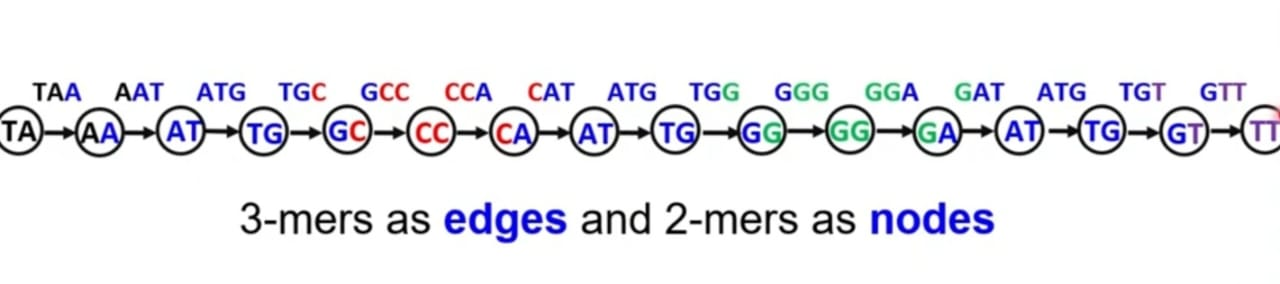
\includegraphics[width=0.8\textwidth]{A.jpeg}
\end{frame}

\begin{frame}{Imagem 2: Pontes de Königsberg}
    \centering
    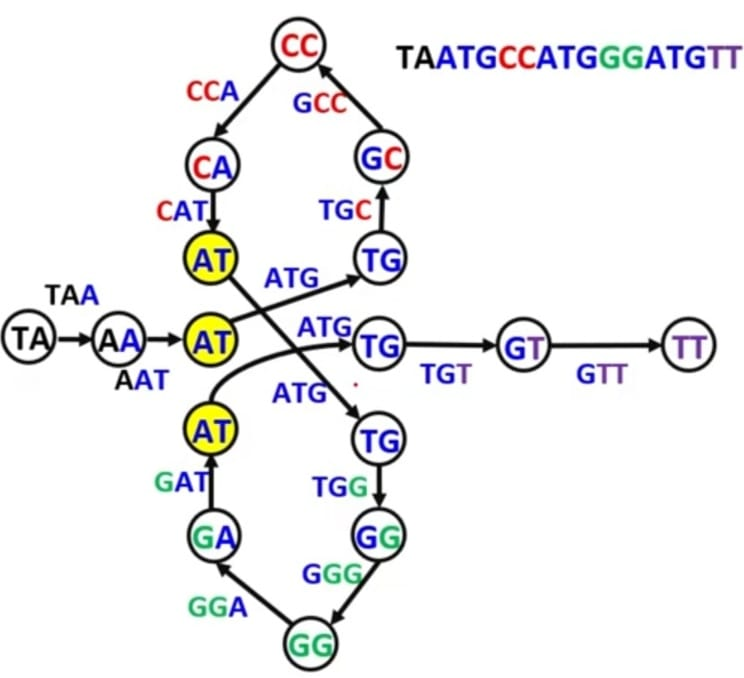
\includegraphics[width=0.8\textwidth]{B.jpeg}
\end{frame}

\begin{frame}{Imagem 3: Fragmentos de DNA}
    \centering
    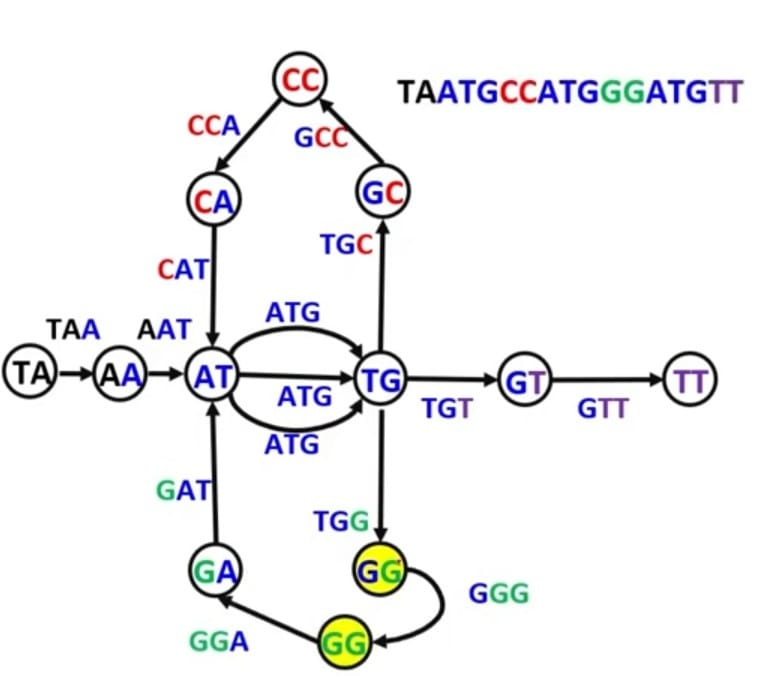
\includegraphics[width=0.8\textwidth]{C.jpeg}
\end{frame}

\begin{frame}{Imagem 4: Caminho Euleriano}
    \centering
    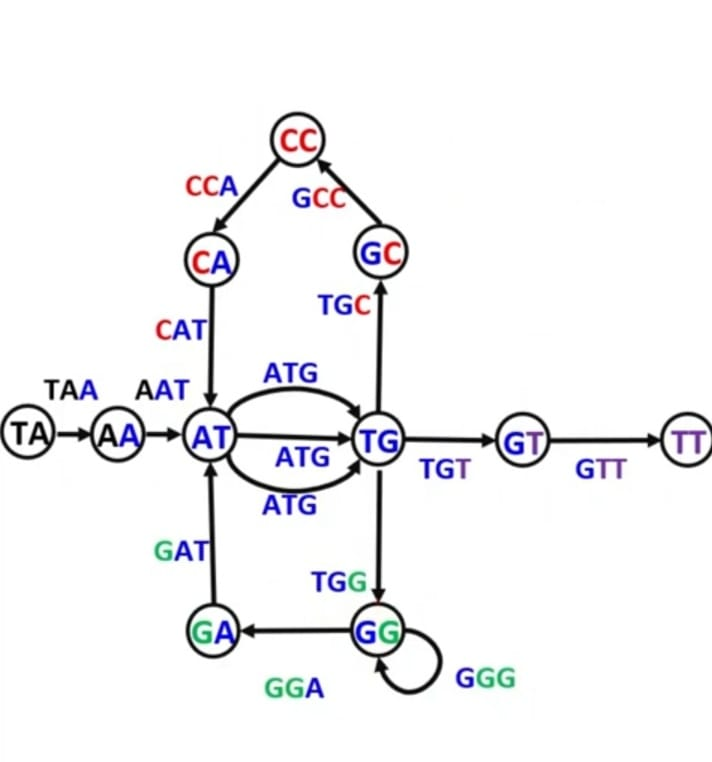
\includegraphics[width=0.8\textwidth]{D.jpeg}
\end{frame}


\begin{frame}{Fim}
\centering
{\Huge Perguntas?\\}
\end{frame}

\end{document}
